\section{Exercício 2}

Data Source:
\begin{itemize}
    \item (info) \url{https://web.stanford.edu/~hastie/ElemStatLearn/datasets/prostate.info.txt}
    \item (database) \url{https://web.stanford.edu/~hastie/ElemStatLearn/datasets/prostate.data}
\end{itemize}

“The data for this example come from a study by Stamey et al. (1989). They examined the correlation between the level of prostate-specific antigen (lpsa) and a number of clinical measures in men who were about to receive a radical prostatectomy. The variables are log cancer volume (lcavol), log prostate weight (lweight), age, log of the amount of benign prostatic hyperplasia (lbph), seminal vesicle invasion (svi), log of capsular penetration (lcp), Gleason score (gleason), and percent of Gleason scores 4 or 5 (pgg45).”

Considere a variável (lpsa) como 'target' e as variáveis (lcavol), (lweight), (age), (lbph), (svi), (lcp), (gleason) e (pgg45) como 'entradas'. Siga o roteiro abaixo:
\begin{enumerate}[label=(\alph*)]
    \item Padronize os atributos de entrada para que eles tenham média 0 e variância 1;
    \item Divida o dataset em dois conjuntos, treinamento e teste, conforme indicado nos índices da última coluna (T = treinamento, F = teste);
    \item Encontre o modelo linear de regressão ótimo no critério de mínimos quadrados (solução LS);
    \item Implemente modelos lineares regularizados pelos métodos 'Ridge' e 'Lasso' que minimizam a função objetivo \( L(w) = \frac{1}{2N} RSS(w) + \lambda ||w||^q \). Apresente resultados para \( \lambda = 0.25 \);
    \item Aplicando as regressões 'Ridge' e 'Lasso' e utilizando k-fold cross-validation, é possível selecionar um valor para \( \lambda \) que resulta em um modelo com melhor capacidade de generalização. Isso é feito selecionando o \( \lambda \) relativo à menor estimativa do erro de predição quadrático médio (usualmente chamado de validation score) ao longo dos k-folds. Também é possível selecionar um valor de \( \lambda \) que seleciona o modelo mais simples dentro de uma tolerância da estimativa do erro de predição quadrático médio. Isso é particularmente útil quando se deseja encontrar soluções esparsas (no caso do Lasso) ou de menor norma L2 (no caso do Ridge). Para tal, um critério comumente adotado é a 'Regra de 1 desvio padrão', onde escolhe-se o maior \( \lambda \) cujo validation score seja igual ou pouco menor do que o 'score mínimo' + '1 desvio padrão do score mínimo'.
    \begin{itemize}[label=-]
        \item Monte as curvas de validation score de k-fold cross-validation em função de \( \lambda \) para os modelos regularizados por 'ridge' e 'lasso' (Sugestão: use k = 10, e procure \( \lambda \) em um intervalo [0, 0.5]);
        \item Calcule o desvio padrão do 'score' mínimo em cada respectiva curva e desenhe-o como barra de erro em torno daquele ponto;
        \item Determine o \( \lambda \) que resulta no modelo mais simples de acordo com a 'Regra de 1 desvio padrão';
        \item Treine o modelo final 'ridge' e 'lasso' utilizando todos os dados (de treinamento) e o respectivo \( \lambda \) encontrado e apresente os resultados;
    \end{itemize}
    \item Utilizando o conjunto de teste construído no item (b), calcule a estimativa do erro de predição quadrático médio do conjunto de teste para cada modelo (mínimos quadrados, 'ridge' e 'lasso'). Disserte sobre os resultados obtidos.
    \item (Bônus) Estime o desvio padrão dos coeficientes do modelo obtido pelo método de bootstrap dos resíduos;
\end{enumerate}

Dica: Veja os slides 9 e 10 de \url{http://www.est.ufmg.br/~cristianocs/MetComput/Aula8.pdf}

\subsection{Resposta do item (a)}
Para padronizar os dados de entrada com média zero e variância um, foram selecionadas as colunas 'lcavol', 'lweight', 'age', 'lbph', 'svi', 'lcp', 'gleason' e 'pgg45' como features e depois utilizada a classe $StandardScaler$ da biblioteca  \textit{sklearn} para \textit{python}, que realiza a padronização dos dados pelo método \textit{z-score}.

\subsection{Resposta do item (b)}
O dataset foi dividido utilizando a última coluna (T = treinamento, F = teste), como pedido no enunciado.

\subsection{Resposta do item (c)}
Para implementar o método dos mínimos quadrados foi utilizada a classe $LinearRegression$ da biblioteca  \textit{sklearn} para \textit{python}.
Pelo critério de mínimos quadrados (LS) foram obtidos os seguintes resultados ao se calcular o erro quadrático médio:

\begin{itemize}
    \item MSE - Treinamento (LS): 0.4391997680583344
    \item  MSE - Teste (LS): 0.5212740055076001
\end{itemize}


\subsection{Resposta do item (d)}
Para implementar o método dos mínimos quadrados foram utilizadas as classe $Ridge$ e $Lasso$ da biblioteca \textit{sklearn} para \textit{python}, ambos utilizando $\lambda=0.25$.
Foram obtidos os seguintes reesultados para cada método ao se calcular o erro quadrático médio:

\begin{itemize}
    \item MSE - Treinamento (Ridge): 0.4392308191154076
    \item MSE - Teste (Ridge): 0.5189192261819305
    \item MSE - Treinamento (Lasso): 0.6207140544187021
    \item MSE - Teste (Lasso): 0.5031909828714028
\end{itemize}

\subsection{Resposta do item (e)}
Para implementar o k-fold cross-validation foi utilizada a classe $KFold$ e o método $cross_val_score$ da biblioteca \textit{sklearn} para \textit{python}, utilizando $k=10$.
As curvas abaixo mostram os resultados para os dois métodos:

\begin{figure}[H]
    \centering
    \caption{Seleção do $\lambda$ para o Ridge}
    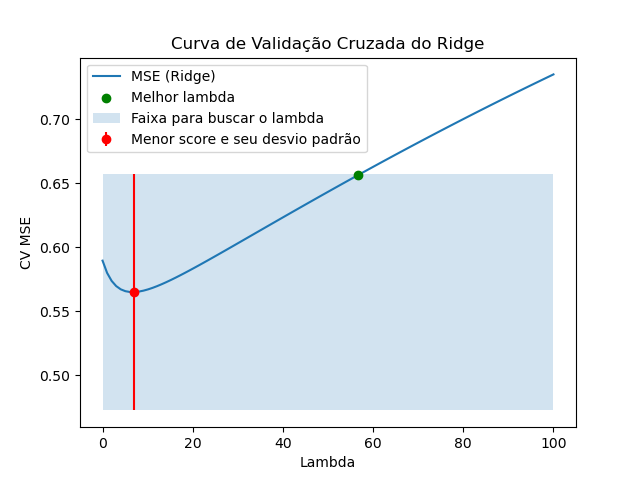
\includegraphics[width=12cm]{ridge.png}
\end{figure}

\begin{itemize}
    \item Best lambda (Ridge): 284.8035868435802
\end{itemize}

\begin{figure}[H]
    \centering
    \caption{Seleção do $\lambda$ para o Lasso}
    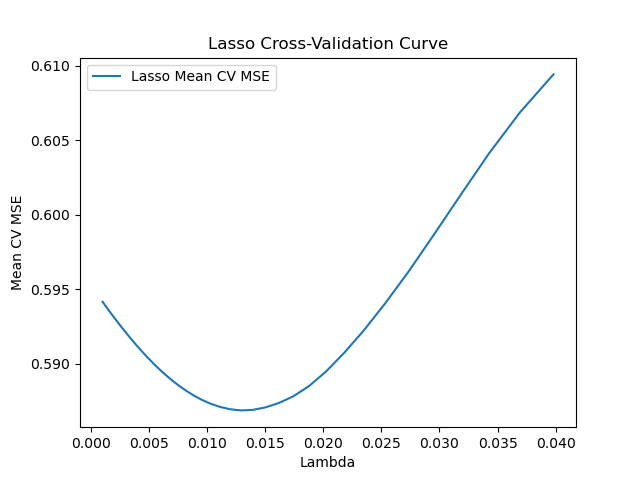
\includegraphics[width=12cm]{lasso.png}
\end{figure}

\begin{itemize}
    \item Best lambda (Lasso): 0.4750810162102798
\end{itemize}

\subsection{Resposta do item (f)}
Utilizando os valores de $\lambda$ obtidos no item (e) para treinar os modelos e avaliando eles no conjunto de teste, foram obtidos os seguintes resultados:

\begin{itemize}
    \item MSE - Teste (Final Ridge): 0.6757602963351064
    \item MSE - Teste (Final Lasso): 0.6427793406214352
\end{itemize}

\subsection{Resposta do item (g) (bônus)}
Estimando-se o desvio padrão dos modelos utilizando o método de bootstrap, como explicado no slide fornecido, foram obtidos os seguintes resultados:

\begin{table}[H]
    \caption{Desvio padrão dos coeficientes estimado pelo método de bootstrap}
    \centering
        \begin{tabular}{|l|lll|}
            \toprule
            Coeficiente & LS & Ridge & Lasso \\
            \midrule
            $\sigma(w_{lcavol})$ & 1.13557895 & 0.02041017 & 0.00122013 \\
            $\sigma(w_{lweight})$ & 0.61004347 & 0.02223836 & 0. \\
            $\sigma(w_{age})$ & 1.4497133 & 0.02089434 & 0. \\
            $\sigma(w_{lbph})$ & 0.80596082 & 0.02063686 & 0. \\
            $\sigma(w_{svi})$ & 1.20836005 & 0.02081217 & 0. \\
            $\sigma(w_{lcp})$ & 2.91104245 & 0.01875707 & 0. \\
            $\sigma(w_{gleason})$ & 1.33500253 & 0.01904607 & 0. \\
            $\sigma(w_{pgg45})$ & 1.21153016 & 0.019532 & 0. \\
            \bottomrule
        \end{tabular}
\end{table}






